\section{Factor Trees}
% Task
% Factor Elimination
% Performance depends on elimination order
% Factor tree with messages
% tree building

\subsection{Task Description}


\begin{frame}
\frametitle{Task Description}
\begin{columns}
\column{.4\textwidth}
\begin{itemize}
\item Exact inference
\item Use elimination trees
\item Prior Marginal, Posterior Marginal \& PoE
\end{itemize}
\column{0.6\textwidth}
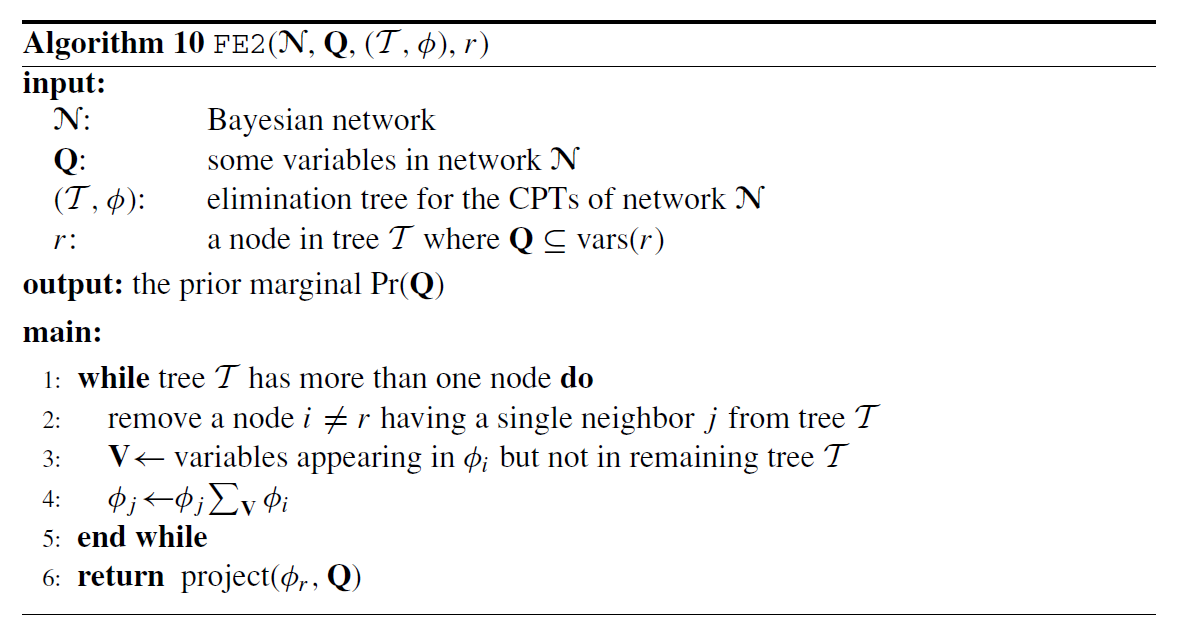
\includegraphics[width=.8\textwidth]{figures/algo10}
\end{columns}
\end{frame}




\subsection{Factor Elimination}



\subsection{Elimination Trees}

\subsection{Building Strategies}


\subsection{Literature}

\begin{frame}
\frametitle{Literature}
\begin{itemize}
\item Modeling and Reasoning with Bayesian Networks , Adnan Darwiche 
\end{itemize}
\end{frame}

\begin{frame}
\textbf{Thank you for your attention!}
\end{frame}

